\deu{\section{Datenanalyse}\index{Datenanalyse}}
\eng{\section{Data analysis}\index{Data analysis}}
\setcounter{aufgabenNummer}{1}
  \renewcommand{\kAufgabenBuchstabe}{D}

\isAufgaben{
\subsection{\deu{Vorbemerkungen}\eng{Preliminaries}}
\deu{\paragraph{Abkürzungen}}\eng{\paragraph{Abbrevations}}

$n$ = Anzahl Werte

$Q_1$ = \deu{erstes Quartil}\eng{first quartile} 


$IQR$ = Interquartilsrange = Quartilsdifferenz (QD) = $Q_3 - Q_1$

\deu{$\varsigma$ = Standardabweichung (Nenner = $n$).}

\eng{$\varsigma$ = Standard Deviation (Denominator = $n$).}

$\overline{x}$ = \deu{empirischer Mittelwert}\eng{average}

$med$ = Median

$Q_3$ = \deu{drittes Quartil}\eng{third quartile} 

$R$ = Range = Spannweite
}




\subsection{\deu{Grundlagen}\eng{Basics}}

\kNiveauAufgabe{
\eng{translate:}

Das Säulendiagramm zeigt die Anzahl Kinder pro Familie in einer Siedlung mit
$n=150$ Familien (10 Familien haben keine Kinder, 25 Familien haben 1
  Kind, ...).

\makebox{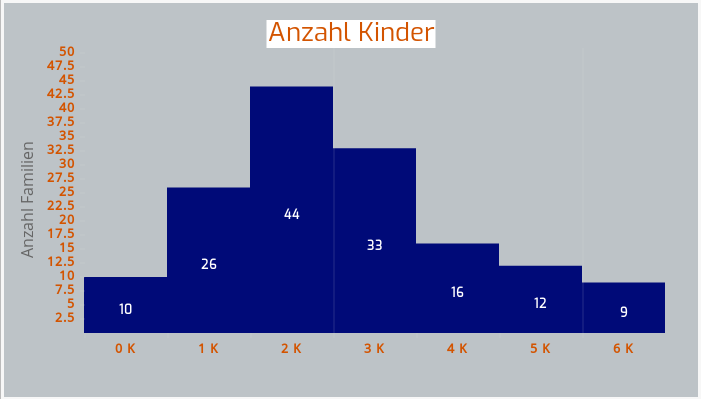
\includegraphics[width=10cm]{img/stoch/statistic_anz_familien_anz_kinder.png}}

a) Berechnen Sie die relativen Häufigkeiten als Dezimalzahl (3
Dezimalen) und in Prozenten (1 Dezimale).

b) Berechnen Sie die durchschnittliche Kinderzahl pro Familie

c) Erklären Sie anhand dieses Beispiels die Begriffe

\textit{Stichprobenumfang\index{Stichprobe}\index{Stichprobenumfang}, Merkmalsträger\index{Merkmalsträger}, Merkmal\index{Merkmal}, Merkmalsprägung\index{Merkmalsprägung},
  absolute Häufigkeit\index{absolute
    Häufigkeit}\index{Häufigkeit!absolute}, relative
  Häufigkeit\index{relative Häufigkeit}\index{Häufigkeit!relative}}

d) Wie viele Kinder leben in dieser Siedlung?
}{% Lösungen
a)

\begin{tabular}{|c|c|c|c|c|c|c|c|}\hline
Anzahl Kinder       & 0      & 1     & 2     &  3    & 4     & 5      & 6   \\\hline
Relative Häufigkeit & 0.063  & 0.173 & 0.293 & 0.220 & 0.107 & 0.080  & 0.060     \\\hline
in \%               & 6.3    & 17.3  & 29.3  & 22.0  & 10.7  & 8.0    & 6.0 \\\hline
 \end{tabular} 

b) $\overline{x} \approx 2.61 $ Kinder pro Familie

c) Siehe Theorie

d) Es leben 391 Kinder in der Siedlung.

}{10}


\kNiveauAufgabe{
\eng{translate:}  Gegeben sind folgende Rohdaten:

  7, 5, 3, 8, 1, 2, 10, 5, 8, 9, 2

  \begin{enumerate}[label=\alph*)]
  \item Erstellen Sie eine geordnete Liste.
  \item Auf welchem Rang\index{Rang} befindet sich der Wert 3?
    \item Welcher Wert befindet sich auf dem mittleren Rang?
  \end{enumerate}
}{%% Lösungen
a) 1 , 2 , 2 , 3 , 5 , 5 , 7 , 8 , 8 , 9 , 10

b) Auf dem 4. Rang.

c) Median: $\mediantilde{x}=5$
}{8}
%%%%%%%%%%%%%%%%%%%%%%%%%%%%%%%%%%%%%%%%%%%%%%%%%%%%%%%%%%%%%%%%%%%%%%%%%%%%%%%%%%%%%%%%%%%%%%%%%%%%%%%%%%%%%%%%%%%%%%555
\subsection{Datenerhebung: Problematik von Ausreißern}

\kNiveauAufgabe{\eng{translate:}
 Das Durchschnittsvermögen in einer kleinen Gemeinde mit 250
  steuerpflichtigen Personen betrug CHF 175\,600.-.

  Durch den Zuzug einer einzigen vermögenden Person erhöhte sich
  dieser Durchschnitt auf CHF 220\,900.-. Wie hoch ist das Vermögen
  dieser Person?
}{%% Lösung
Das Vermögen dieser Person ist etwa CHF $11\,545\,900.--$
}{8}


\kNiveauAufgabe{\eng{translate:}
Das monatliche Durchschnittseinkommen in einer Firma mit 850
  Beschäftigten beträgt CHF 7\,250.-. Die drei Spitzenverdiener dieser
  Firma verdienen monatlich je CHF 86\,000.-.
  Berechnen Sie das monatliche Durchschnittseinkommen, wenn diese drei
  Spitzenwerte nicht berücksichtigt werden.
}{%% Lösung
Pro nicht-Spiztenverdiener sind das CHF $6\,971.05$.
}{8}

\kTrainingAufgabe{\eng{translate:}
In einer Schulklasse ergaben sich bei der Auswertung einer Prüfung
  folgende Punktezahlen:

  35, 58, 59, 4, 38, 43, 45, 52, 49, 55

  a) Berechnen Sie Mittelwert und Median.

  b) Berechnen sie den Mittelwert ohne den Ausreißer 4.
}{%% Lösung
Taschenrechner:

 a) Mittelwert $\overline{x} =  43.8$ und Median $\mediantilde{x} = 47 $

 b) Mittelwert $\overline{x} =  48.\overline{2}$

}{8}

\kNiveauAufgabe{\eng{translate:}
  10 Eier haben folgende Gewichte in Gramm:

  52.8, 55.9, 58.2, 57.1, 60.4, 69.1 57.9, 58.0, 62.5, 65.0

  Nun wird aus Jux zu den Eiern ein Gips-Ei hinzugelegt. Dadurch
  erhöht sich das Durchschnittsgewicht um 3.48 Gramm pro Ei.

  Berechnen Sie das Gewicht des Gips-Eies.

  Runden Sie auf 0.1 Gramm genau.
}{%% Lösung
Das Gips-Ei wiegt 98.0 g.
}{8}
\newpage

\subsection{Diagramme (Säulendiagramm, Histogramm, Boxplot)}


\kNiveauAufgabe{
\textbf{Säulendiagramm}

  In einer Ausstellung wurden im Laufe einer Woche folgende
  Besucherzahlen ermittelt:

  \begin{tabular}{ccccccc}
    Montag & Dienstag & Mittwoch & Donnerstag & Freitag & Samstag & Sonntag \\
    350    & 321      & 647      & 519        & 844     & 1\,314  & 2\,522
  \end{tabular}

  Zeichnen Sie ein \textbf{Säulendiagramm} mit den relativen
  Häufigkeiten in \%.

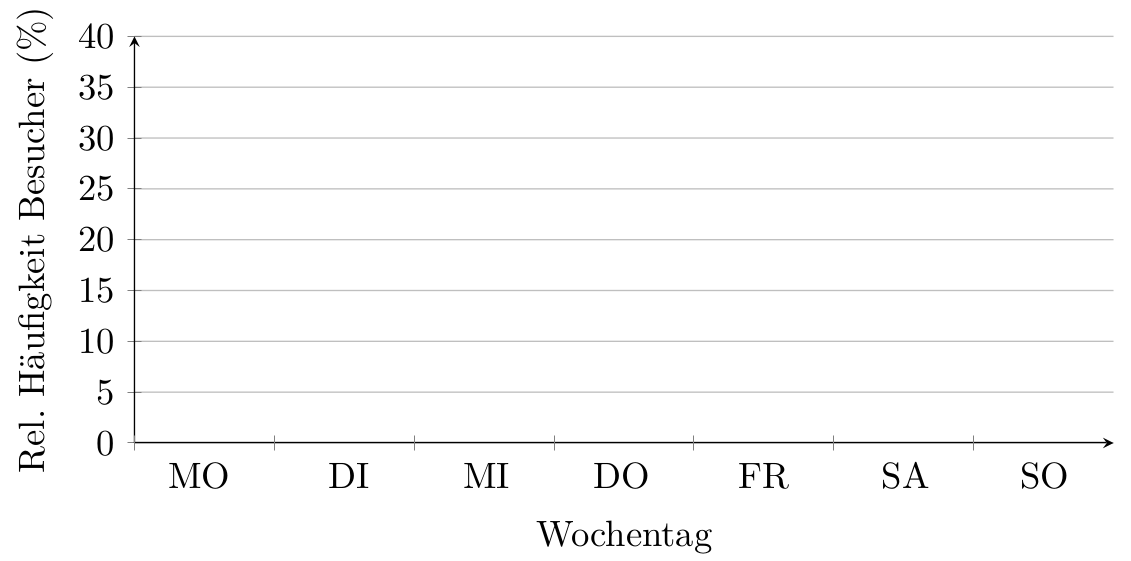
\includegraphics[width=120mm]{img/daan/Museum_Aufgabe.png}

}{%% Lösung
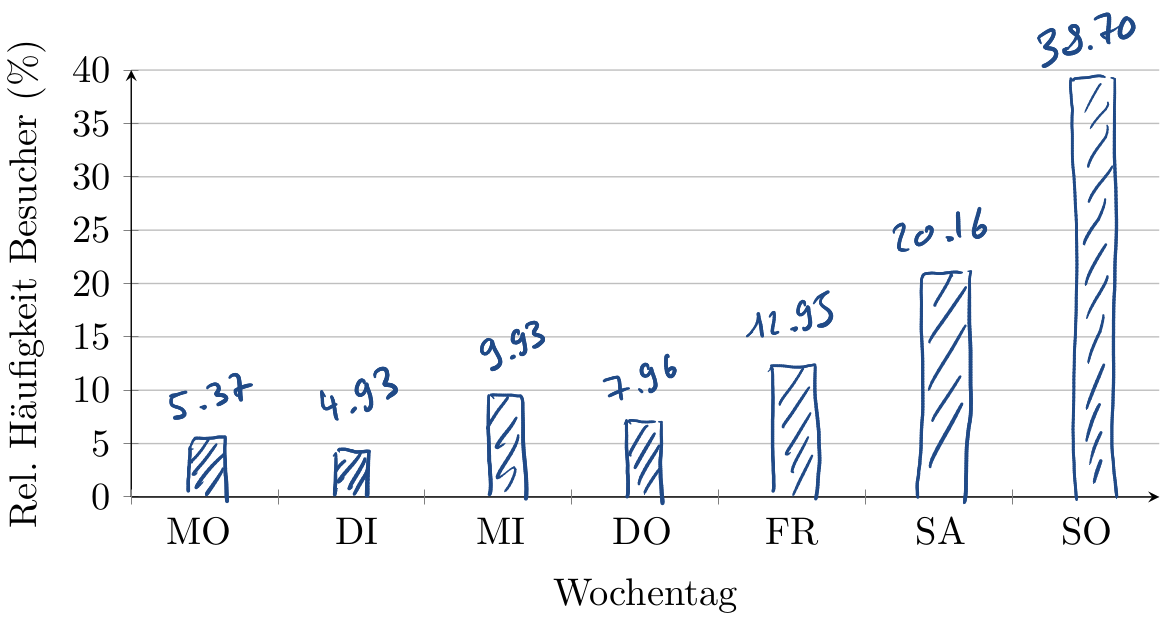
\includegraphics[width=120mm]{img/daan/Museum_Loesung.png}
}{8}
\newpage






\kNiveauAufgabe{
 \textbf{Säulendiagramm und Boxplot}

  Hier sehen Sie die Prüfungspunkte in einer Klasse.

  Geordnete Urliste:

  52, 62, 66, 72, 74, 74, 76, 76, 76, 78, 80, 82, 82, 84, 86, 88, 92, 96

  \begin{enumerate}[label=\alph*)]
      \item
        Bestimmen Sie die \textbf{Quartilsdifferenz} \textit{IQR}.
      \item
    Teilen Sie die Daten in Klassen ein: $[50; 60[$, $[60; 70[$, usw.
        \textit{(Klassenbreite = 10 Punkte).} Zeichnen Sie ein
        Histogramm mit den relativen Häufigkeiten. 
      \item
        Zeichnen Sie einen \textbf{Boxplot}.
      \item
        Bestimmen Sie den \textbf{Mittelwert}.
      \item
        Bestimmen sie den \textbf{Modalwert} (Modus).
    \end{enumerate}
%%    \mmPapierZwei{6}{17.5}
\begin{tabular}{c}
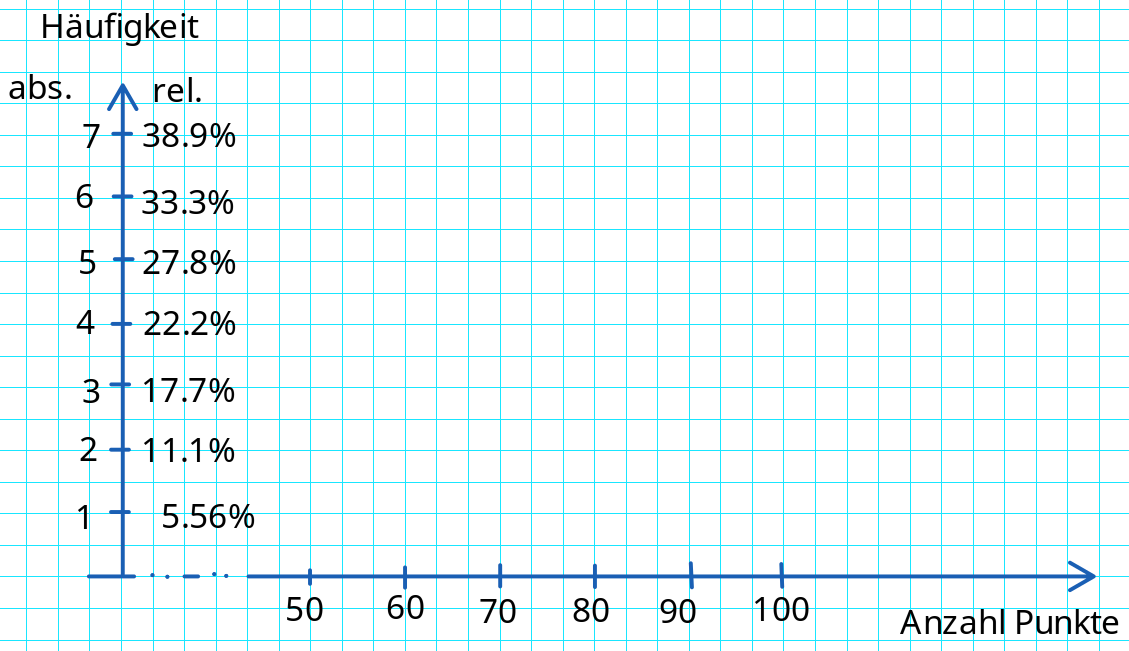
\includegraphics[width=100mm]{img/daan/HistogrammLeer.png} \\
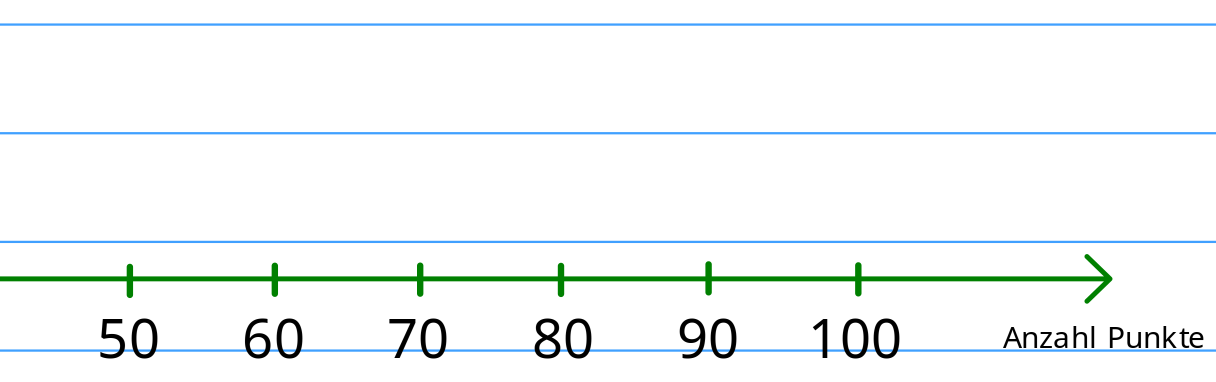
\includegraphics[width=120mm]{img/daan/BoxplotLeer.png}
 \end{tabular}
\newpage 
}{%% Lösung
a) Median = 76.5; Q1 = 74;  Q3 = 84 und IQR(=QD)=10

   Maximale Whisker-Länge ist somit 15 und die obere Ausreisserschwelle
   liegt bei 99 und die untere Ausreisserschwelle bei 59. Somit ist
   nur unten ein Ausreißer zu finden.
   
b) c)

\begin{tabular}{cc}
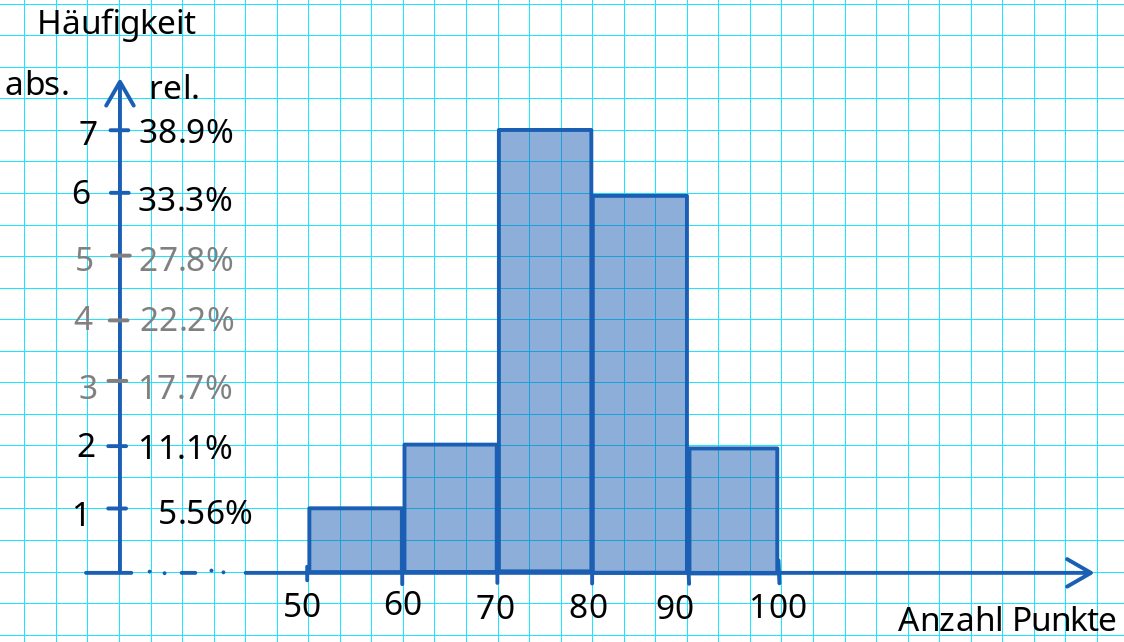
\includegraphics[width=88mm]{img/daan/HistogrammVoll.png} & 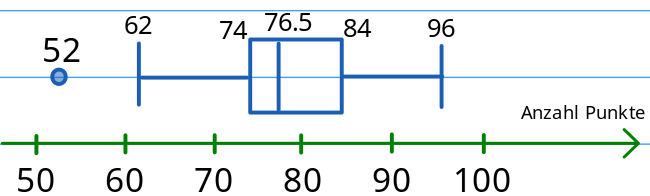
\includegraphics[width=74mm]{img/daan/BoxplotVoll.png}
 \end{tabular}

d) Summe = 1396. Mittelwert = 77.555.. Punkte

e) Der Modus ist 76, die Zahl kommt drei mal vor.
}{8}










\kNiveauAufgabe{
\textbf{Klassendiagramm, Säulendiagramm, Boxplot}
 Die Messung der Körpergrösse von 100 18-jährigen Schülern liefert
 folgende Zahlen:

 \begin{tabular}{lcccccccccc}
   Grösse in cm & 163 & 164 & 165 & 166 & 167 & 168 & 169 & 170 & 171 & 172\\
   Anzahl      &  1  &  1  &  1  &  3  &  3  &  3  &  4  &  6  &  5  &  5
   \end{tabular}

 \begin{tabular}{lcccccccccc}
   Grösse in cm & 173 & 174 & 175 & 176 & 177 & 178 & 179 & 180 & 181 & 182\\
   Anzahl      &  4  &  7  &  6  &  5  &  5  &  7  &  5  &  4  &  4  &  6
   \end{tabular}

  \begin{tabular}{lcccccc}
   Grösse in cm & 183 & 184 & 185 & 186 & 187 & 188\\
   Anzahl      &  5  &  3  &  3  &  2  &  1  &  1 
  \end{tabular}

  \begin{enumerate}[label=\alph*)]
  \item Erstellen Sie eine Klasseneinteilung mit Klassenbreite 5cm:

    Klasse 1: [160cm; 165cm[

    Klasse 2: [165cm; 170cm[

        usw.

        Zeichnen Sie anschliessend ein Histogramm mit den relativen
        Häufigkeiten in Prozent.

        \item Zeichnen Sie einen Boxplot mit diesen Daten.
\end{enumerate}
}{%% Löusngen

\begin{tabular}{c|c|c|c|c|c|c}
[160;165[ & [165;170[ & [170;175[ & [175;180[ & [180;185[ & [185;190[  & $\Sigma$ \\\hline
    1     &     2     &     8     &    5      &     2     &   18       &     36\\\hline
    2\%   & 14\%      & 27\%      & 28\%      &22 \%      & 7\%       & 100\%\\
 \end{tabular}
 
\begin{tabular}{cc}
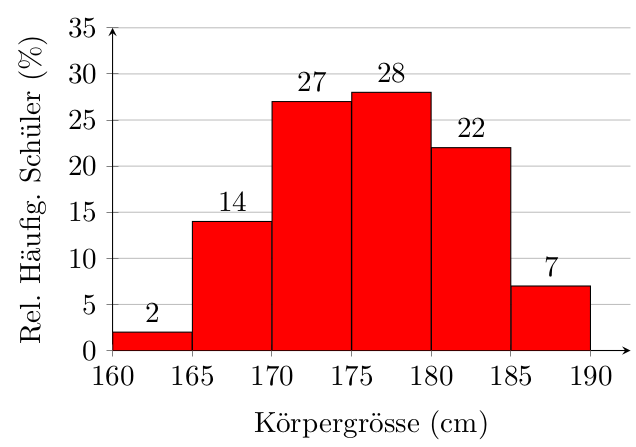
\includegraphics[width=70mm]{img/daan/KoerpergroesseHistogramm.png}
&
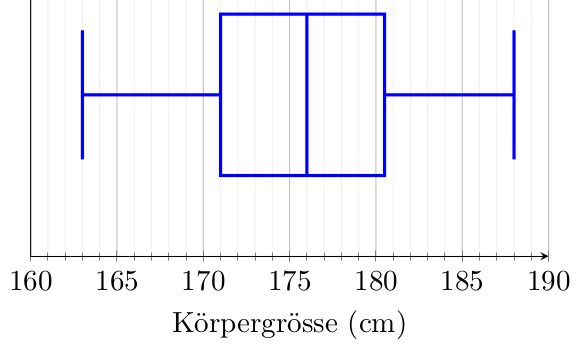
\includegraphics[width=80mm]{img/daan/KoerpergroesseBoxplot.png}
\end{tabular}
}{8}
\newpage











\kNiveauAufgabe{
\textbf{Vergleich zweier Boxplots}
  Wurfweiten beim Ballwurf in Metern:

  Versuchsreihe 1:

  34.0, 34.4, 32.2, 33.5, 35.2, 32.9, 32.6, 34.3, 33.2, 34.1,
  33.2, 33.2, 34.0, 32.7. 34.8, 33.5, 33.5

  Versuchsreihe 2:

  32.8, 33.7, 34,9, 34.3, 34.6, 32.3, 34.0, 33.9, 33.0, 32.4,
  31.1, 35.5, 31.7, 34.8, 33.5, 32.4

  Erstellen Sie für beide Versuchsreihen je einen Boxplot (Darstellung
  mit gleicher Skala, sodass ein Vergleich möglich wird).
}{%% Lösungen
V1: Q1 = 33.05; Median = 33.5; Q3 = 34.2

V2: Q1 = 32.4; Median = 33.6; Q3 = 34.5

Zahlen unbedingt nochmals prüfen, denn die Graphik stimmt nicht (V1
mit V2 tauschen, Q1 und Q3 nochmals kontrollieren, Mittelachse löschen)...

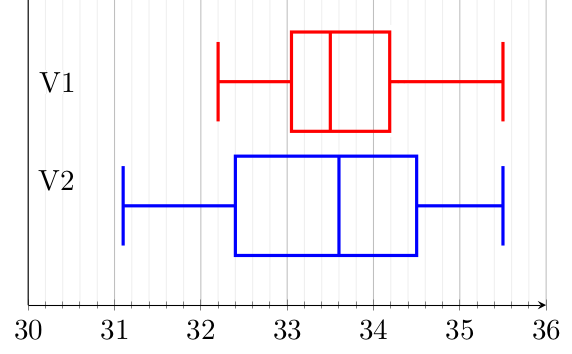
\includegraphics[width=120mm]{img/daan/VergleicheZweiBoxplots.png}

}{8}
\newpage







\kNiveauAufgabe{
\textbf{Informationen aus einem Diagramm herauslesen}
Praliné-Kugeln in einer Packung; Darstellung der absoluten
Häufigkeiten in g. Bestimmen Sie
Mittelwert, Median und Standardabweichung. Rechnen Sie mit den Klassenmitten.

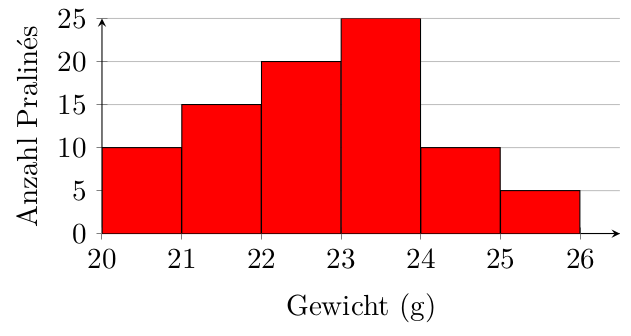
\includegraphics[width=120mm]{img/daan/HistogrammPralines.png}
    
%\begin{tikzpicture}\begin{axis}[ybar stacked,nodes near coords,bar
%    width=0.4,]\addplot
%    coordinates{(21,10) (22,15) (23, 20) (24, 25) (25, 10) (26, 5)};\end{axis}\end{tikzpicture}

Bestimmen Sie Mittelwert, Median und Standardabweichung.

}{%% Lösungen
$\overline{x} = 28.8$, $\mediantilde{x}=22.5$ und $\sigma=1.4$.


}{8}

\newpage














\subsubsection{Masszahlen (Mittelwert, Media, Quartile,
  Standardabweichung, Quartilsdifferenz)}

\kNiveauAufgabe{
\eng{translate:} In einer Klasse wurden folgende 18 Prüfungsnoten erzielt:

  \begin{tabular}{llllllllll}
    3 & 3 & 3.5 & 3.5 & 4   & 4 & 4.5 & 4.5 & 4.5 & 4.5\\
    5 & 5 & 5.5 & 5.5 & 5.5 & 6 & 6   & 6
  \end{tabular}

  Berechnen Sie \textbf{Mittelwert} und \textbf{Standardabweichung}
  mit Hilfe des Rechners.
}{%% Lösungen
$\overline{x} = 4.64$, $\sigma=0.97$ (bzw. $s_x=1.0$)
}{8}





\kNiveauAufgabe{
\eng{translate:} Drei \textbf{Streumasse}: \textbf{Spannweite R (Range)},
  \textbf{Quartilsdifferenz IQR}, \textbf{Standardabweichung $\sigma$}

  Gegeben sind folgende Daten, die bereits geordnet sind:

  \begin{tabular}{llllllllll}
    2.5 & 2.8 & 3.2 & 3.5 & 3.5 & 4.1 & 4.2 & 4.7 & 4.8 & 4.8\\
    5.4 & 5.5 & 6
  \end{tabular}

  Ermitteln Sie die \textbf{Spannweite (Range)}, die
  \textbf{Quartilsdifferenz QD (Interquartilerange (IQR)) } und die \textbf{Standardabweichung} (auf
  2 Dezimalen genau).
}{%% Lösungen
Spannweite (Range) = $3.55$, IQR (QD) = $1.75$ und  $\sigma=1.04$ (bzw. $s_x=1.09$)
}{8}
  

\newpage
